\chapter{Technische Charakteristiken und Spezifikationen}

\section{Allgemeines Design und technische Voraussetzungen}
\subsection{Hardware}
Die Hardware besteht aus einem RFID Lesegerätes mit 2 angeschlossenen Antennen. Eine der Beiden Antennen soll sich rund 60cm weiter entfernt befinden und sich direkt neben dem Förderband befinden. Die Zweite Antenne soll sich rund 50cm über dem Förderband befinden und direkt nach unten ausgerichtet sein. Zur Abschirmung zwischen dem Förderband, auf welchem die Tags gemessen werden sollen und dem dahinter befindlichen soll zwischen den beiden Förderbänder eine einfache Aluminium Platte befestigt werden (Siehe \ref{fig:positionAntennen}).

Die Platzierung der Antennen steht in direktem Einfluss mit der Lesbarkeit der Tags, da die Ausrichtung der Tags zur Antenne dazu führen können, dass dieser nicht gelesen werden kann.

\begin{figure}
	\centering
	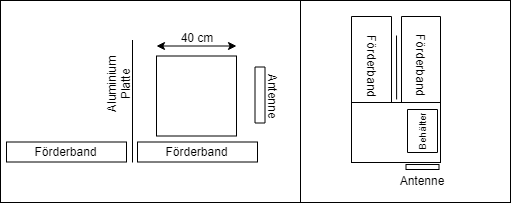
\includegraphics[keepaspectratio,width=\linewidth]{Positionierung_Antennen}
	\caption{Antennenposition eins und zwei}
	\label{fig:positionAntennen}
\end{figure}


Durch die Ausrichtung der Antennen wird weiter vorausgesetzt, dass das Lesegerät mit den Antennen eine maximale Distanz von 53.85cm lesen können. Jeder Behälter enthält gemäss angaben im Normalfall 50 Exemplare, daraus ergibt sich, dass das Lesegerät für den Normalfall mindestens 50 Exemplare in der Zeit auslesen muss, welche das Förderband benötigt um die Kiste ca. 60cm weit zu Transportieren.

\section{Vergleich der vorgeschlagenen Lösung und der existierenden Situation}
Die Existierende Situation enthält momentan noch keine Möglichkeit der Verifikation des Inhaltes eine Behältnisses. Demnach würde durch die Durchführung dieses Projektes die Wahrscheinlichkeit des Deplatzieren massiv verringern.

\section{Vorteile und deren Gründe der vorgeschlagenen Lösung}
\begin{itemize}
	\item Durch die Rückbeziehung welche mittels der Mehrheit der gelesenen Tags auf die ID des Behälter zulässt, kann auf ein Barcodeleser verzichtet werden. Dies ermöglicht eine Positionsunabhängige Erkennung des Behälters.
	\item Die direkte Aussortierung des Behälters bringt mehrere Vorteile. So wird bereits der bestehende Prozess, mit welchem die Mitarbeiter vertraut sind, verwendet. Dies führt weiter zu dem Umstand, dass keine weiteren Fehlerquellen durch zusätzliche manuelle Interaktion durch einen Mitarbeiter, entstehen. Ein weiterer Vorteil liegt darin, dass die Erkennung sehr Früh geschieht, da die Aussortierung noch vor der Einlagerung des Behälters stattfindet.
	\item Der Einsatz mehrerer Antennen bringt den Vorteil, dass Tags mit verschiedenen Ausrichtungen identifiziert werden können. Dies aus dem Grund, dass sich die Tags bei unterschiedlichen Ausrichtungen unterschiedlich stark beeinflussen. Weiter durch den Einsatz mehrere Antennen, der Suchradius vergrössert werden. Dies führt zu dem Umstand, dass sich der Behälter länger in einem Suchradius befindet, wodurch mehr Zeit für die Inventarisierung der Tags zur Verfügung steht. Deshalb können auch mehr Tags gefunden werden.
	\item Die Installation der RFID Antennen soll unmittelbar bei der Waage erfolgen. Dies bringt den Vorteil, dass mehr Zeit für die Inventarisierung zur Verfügung steht, da der Behälter für eine kurze Zeit auf der Waage still steht. Weiter ist mit keiner Interferenz durch andere Behälter, sowie durch weitere Objekte, wie metall, zu rechnen, da nicht sich nur Luft zwischen er Antenne und dem Behälter befindet.
\end{itemize}


\section{Vorgeschlagene Zulieferungsquellen}

\section{Geschätzte Kosten und Quellen für die Basis dieser Schätzungen}
